% Fig 1 — QP-Faith pipeline schematic (EDITABLE SOURCE).
% Compile: pdflatex fig1_pipeline.tex  -> fig1_pipeline.pdf
% Then copy the pdf into submission_ipm/.  Kept as source so the labels can be
% edited in future (the previous fig1 was a source-less PDF whose "hallucinated"
% label contradicted the paper's "not hallucination... mis-routing" framing).
\documentclass[border=8pt]{standalone}
\usepackage{tikz}
\usetikzlibrary{arrows.meta, positioning, fit, calc}
\begin{document}
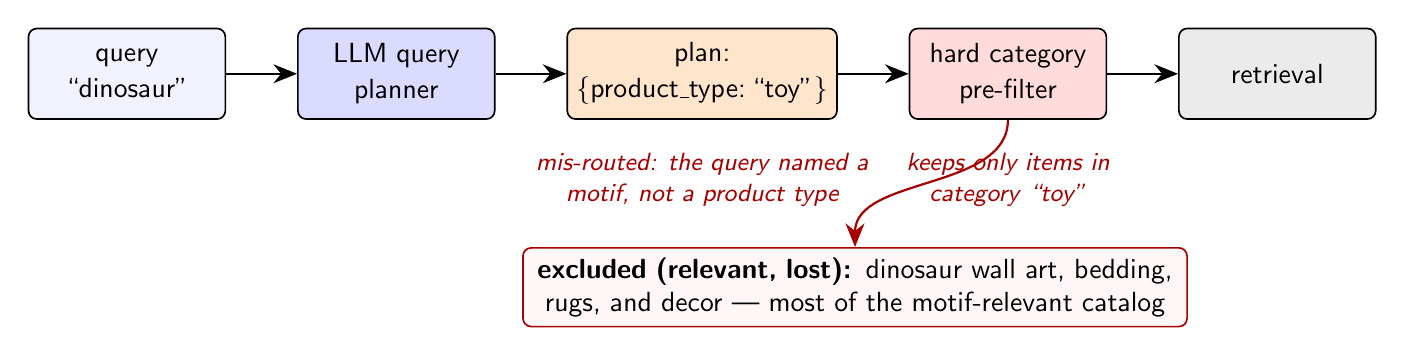
\begin{tikzpicture}[
  font=\sffamily,
  box/.style={draw, rounded corners=3pt, minimum height=1.15cm, minimum width=2.5cm,
              align=center, line width=0.6pt},
  arr/.style={-{Stealth[length=3mm,width=2.4mm]}, line width=0.8pt},
  node distance=9mm,
]
% --- pipeline row ---
\node[box, fill=blue!5]                       (q)    {query\\[1pt]``dinosaur''};
\node[box, fill=blue!14, right=of q]          (plan) {LLM query\\[1pt]planner};
\node[box, fill=orange!20, right=of plan]     (out)  {plan:\\[1pt]\{product\_type:\,``toy''\}};
\node[box, fill=red!14, right=of out]         (filt) {hard category\\[1pt]pre-filter};
\node[box, fill=black!8, right=of filt]       (ret)  {retrieval};
\draw[arr] (q) -- (plan);
\draw[arr] (plan) -- (out);
\draw[arr] (out) -- (filt);
\draw[arr] (filt) -- (ret);

% --- the failure, annotated under the plan the planner emits ---
\node[below=3mm of out, text=red!65!black, align=center, font=\sffamily\small\itshape]
  (mr) {mis-routed: the query named a\\ motif, not a product type};
\node[below=3mm of filt, text=red!65!black, align=center, font=\sffamily\small\itshape]
  (kp) {keeps only items in\\ category ``toy''};

% --- excluded set, spanning under the emit/filter region ---
\node[draw=red!65!black, rounded corners=3pt, line width=0.6pt, fill=red!3,
      align=center, minimum height=1cm, text width=8.2cm,
      below=22mm of $(out)!0.5!(filt)$] (exc)
  {\textbf{excluded (relevant, lost):} dinosaur wall art, bedding,\\ rugs, and decor --- most of the motif-relevant catalog};
\draw[arr, red!65!black] (filt.south) .. controls +(0,-0.9) and +(0,0.9) .. (exc.north);
\end{tikzpicture}
\end{document}
